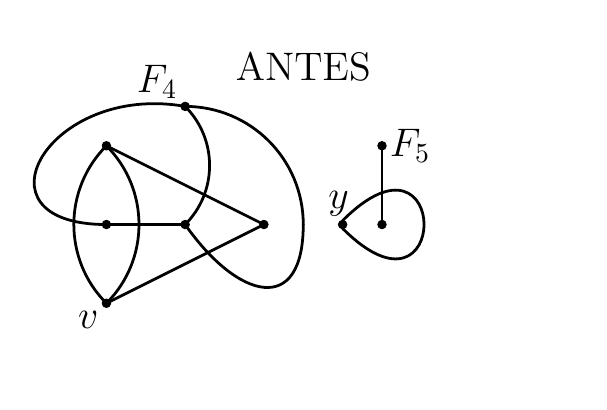
\begin{tikzpicture}[line cap=round,line join=round,x=1cm,y=1cm]
\clip(-1,-1) rectangle (6,3.5);


\draw [line width=1pt] (0,0) to[in=-135,out=135,looseness=1]  (0,2); % v -- u
\draw [line width=1pt] (0,0) to[in=-45,out=45,looseness=1]  (0,2);   % v -- u
\draw [line width=1pt] (2,1) to  (0,0); % 4 -- 6
\draw [line width=1pt] (2,1) to  (0,2); % 4 -- 6
%\draw [line width=1pt] (2,1) to  (3,1); % 4 -- 6
\draw [line width=1pt] (3,1.05) to[out=45,in=-45,looseness=50] (3,.95); % 4 -- 4


\draw [line width=1pt] (1,2.5) to[out=-45,in=45,looseness=1] (1,1); % c: F0 -- F1
\draw [line width=1pt] (1,2.5) to[out=0,in=90,looseness=1] (2.5,1); % d: F0 -- F1
\draw [line width=1pt] (1,1) to[out=-55,in=-90,looseness=2] (2.5,1); % d: F0 -- F1


% laço F0 para F0
%\draw [line width=1pt] (1,2.5) to[out=-30,in=90,looseness=1] (2.5,1); % F0 -- F1
%\draw [line width=1pt] (2.5,1) to[out=-90,in=-90,looseness=2] (4.5,1); % F0 -- F1
%\draw [line width=1pt] (1,2.5) to[out=0,in=90,looseness=1] (4.5,1); % F0 -- F1


\draw [line width=1pt] (1,2.5) to[out=170,in=180,looseness=2.5] (0,1); % F0 -- F2
\draw [line width=1pt] (3.5,2) to (3.5,1); % F0 -- F3
\draw [line width=1pt] (1,1) to (0,1); % F1 -- F2



\draw (2.5,3) node {\Large ANTES};

\begin{scriptsize}
\draw [fill=black] (0,2) circle (1.5pt);
%\draw (0,2) node[anchor=south east] {\Large $u$};


\draw [fill=black] (0,0) circle (1.5pt);
\draw (0,0) node[anchor=north east] {\Large $v$};
\draw [fill=black] (2,1) circle (1.5pt);
%\draw (1.95,1) node[anchor=south] {\Large $z$};
\draw [fill=black] (3,1) circle (1.5pt);
\draw (2.95,1) node[anchor=south] {\Large $y$};


\draw [fill=black] (1,2.5) circle (1.5pt);
\draw (1,2.5) node[anchor=south east] {\Large $F_4$};
\draw [fill=black] (1,1) circle (1.5pt);
%\draw (1,1) node[anchor=west] {\Large $F_1$};
\draw [fill=black] (0,1) circle (1.5pt);
%\draw (0,1) node[anchor=south] {\Large $F_2$};
\draw [fill=black] (3.5,1) circle (1.5pt);
%\draw (3.5,1) node[anchor=west] {\Large $F_3$};
\draw [fill=black] (3.5,2) circle (1.5pt);
\draw (3.5,2) node[anchor=west] {\Large $F_5$};

%\draw (-0.5,1.05) node[anchor=north] {\Large $a$};
%\draw (-0.5,1.1) node[anchor=north] {\Large $2$};

%\draw (0.5,1.35) node[anchor=north] {\Large $b$};
%\draw (0.5,1.05) node[anchor=north] {\Large $7$};

%\draw (1.15,1.7) node[anchor=north] {\Large $c$}; % u -- w
%\draw (1.4,1.7) node[anchor=north] {\Large $3$}; % u -- w

%\draw (1.1,.6) node[anchor=north] {\Large $d$}; % v -- w
%\draw (1.2,.65) node[anchor=north] {\Large $1$}; % v -- w

%\draw (2.3,1.3) node[anchor=north] {\Large $e$}; % v -- w
%\draw (2.3,.95) node[anchor=north] {\Large $4$}; % v -- w

%\draw (4.15,1) node {\Large $f$}; % w -- w
%\draw (4.15,1) node {\Large $2$}; % w -- w

\end{scriptsize}
\end{tikzpicture}
